\chapter{Dati Iniziali}

In questa sezione ci si soffermerà in quella che è una preliminare analisi dei dati iniziali a disposizione. Questi dati rappresentano il materiale grezzo dal quale \textit{estrarre} --- fare del \textit{mining}, come appunto il nome dell'attività suggerisce --- delle informazioni. \\

Usando come metafora una lavorazione meccanica, avere ben chiara la natura del materiale grezzo a disposizione consente di scegliere opportunamente gli utensili adatti per il lavoro da fare. Nel nostro caso, poter vantare di una comprensione generale di ciò che si ha a disposizione, potrà consentirci di scegliere le tecniche migliori per trarre il meglio dai dati iniziali. \\

\section{Carriera degli Studenti}

Una parte fondamentale dell'analisi descritta in questo lavoro è basata su questo dataset, rappresentante i dati riguardanti la produttività di tre coorti d'immatricolazione di studenti in un periodo di quattro anni. Più nel dettaglio, il dataset si compone di:

\begin{itemize}
	\item \textbf{Coorte 2010}: studenti immatricolati nel 2010, carriera registrata fino all'\textbf{A.A. 2013-2014} compreso
	\item \textbf{Coorte 2011}: studenti immatricolati nel 2011, carriera registrata fino all'\textbf{A.A. 2014-2015} compreso
	\item \textbf{Coorte 2012}: studenti immatricolati nel 2012, carriera registrata fino all'\textbf{A.A. 2015-2016} compreso
	\item \textbf{Coorte 2013}: studenti immatricolati nel 2013, carriera registrata fino all'\textbf{A.A. 2016-2017} compreso
\end{itemize}

Quindi, si ha a disposizione una finestra temporale di risultati ottenuti nei corsi così composta:

\begin{center}
	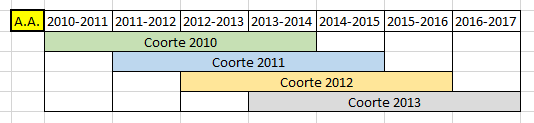
\includegraphics[scale=0.7]{../raw/stud_comp.png}
\end{center}

Questo fatto porta ovviamente ad avere una mole d'informazioni più addensata nella parte centrale della nostra finestra temporale, avendo idealmente dati riguardanti tutte le materie del C.d.L. solo nell'Anno Accademico 2013-2014. Questo aspetto sarà rilevante nell'interpretare i risultati di alcune analisi effettuate in seguito.

\subsection{Formato e Rappresentazione}

Il dataset è stato fornito in un unico file CSV, un formato \textit{plain text} facilmente manipolabile e interpretabile da un'ampia gamma di software. Esso si compone di una unica tabella, nella quale ogni tupla identifica uno studente, per il quale sono presenti attributi che descrivono la sua carriera universitaria nel periodo preso in esame. Oltre alle informazioni generali, quali ad esempio i risultati conseguiti nel test d'ingresso e il numero di crediti totali ottenuti nella finestra temporale esaminata, sono presenti attributi relativi alla data e al voto ottenuto in ciascun esame sostenuto. \\

Nel dettaglio, per ogni tupla rappresentante uno studente sono presenti le seguenti informazioni:

\begin{itemize}
	\item \textbf{Coorte} di immatricolazione: $$ \{2010, 2011, 2012, 2013\} $$
	\item Voto conseguito nel \textbf{test di ingresso}: $$ \{ x \in \mathbb{N} \text{ tale che } 0 \leq x \leq 25\} $$
	\item Voto ottenuto all'\textbf{esame di maturità}: $$ \{ x \in \mathbb{N} \text{ tale che } 60 \leq x \leq 100\} $$
	\item Tipo di \textbf{scuola superiore} frequentata: $$ \{LS, LC, IT, TC, IP, AL \} $$ che rappresentano rispettivamente le seguenti cateogrie di scuola superiore: Liceo Scientifico, Liceo Classico, Istituto Tecnico, Istituto Commerciale, Istituto Professionale, Altro
	\item \textbf{Crediti totali} ottenuti: $$ \{ x \in \mathbb{N} \text{ tale che } 0 \leq x \leq 180\} $$
	\item \textbf{Crediti} ottenuti da esami \textbf{con voto}: $$ \{ x \in \mathbb{N} \text{ tale che } 0 \leq x \leq 159\} $$
	\item \textbf{Voto medio} ottenuto negli esami: $$ \{ x \in \mathbb{N} \text{ tale che } 18 \leq x \leq 31 \text { con 31 indicante il 30 con lode}\} $$
	\item \textbf{Voto} ottenuto in un \textbf{certo esame}: $$ \{ x \in \mathbb{N} \text{ tale che } 18 \leq x \leq 31 \text { con 31 indicante il 30 con lode}\} $$
	\item \textbf{Data} in cui è stato sostenuto quell'esame: $$ \text{data in formato }MM/GG/YYYY $$
\end{itemize}

Di tutte queste informazioni, solo parte di esse sono state utilizzate in qualche analisi di \textit{data mining}, come si vedrà meglio nelle sezioni successive.

\subsection{Mole di dati}

Il dataset si compone di 208 record, ognuno dei quali ha 47 attributi. Il file che lo memorizza pesa circa 45 kb. Non si può quindi parlare propriamente di \textit{big data} in questo caso.

\section{Valutazione degli Insegnamenti}

Al fine d'integrare i dati precedenti ponendo l'attenzione sui vari corsi che compongono il C.d.L, sono stati forniti i dati relativi alla valutazione dei corsi di studi da parte degli studenti. Questi dati sono ottenuti da questionari anonimi, che devono essere obbligatoriamente compilati prima di potersi prenotare per un esame. I risultati sono poi divulgati in forma aggregata, garantendo così l'anonimato dello studente. A ogni domanda lo studente ha potuto rispondere indicando un valore compreso fra zero e dieco, con zero a indicare una risposta totalmente negativa e dieci a indicare invece una risposta totalmente positiva.\\

Volendo scendere in un maggior dettaglio, sono stati forniti i dati riguardanti i seguenti anni accademici:

\begin{itemize}
	\item 2010-2011
	\item 2011-2012
	\item 2012-2013
	\item 2013-2014
	\item 2014-2015
	\item 2015-2016
	\item 2016-2017
\end{itemize}

Come si può facilmente notare, la finestra temporale coperta da questi dati va a combaciare con quella trattata dal dataset relativo alla carriera degli studenti. Questo aspetto fondamentale ha permesso di effettuare una operazione di \textit{join} di qualche sorta fra i due dataset a disposizione, che verrà in seguito descritta nella sezione dedicata al \textit{preprocessing}.

\subsection{Formato e Rappresentazione}

Il dataset è stato fornito in sette diversi file CSV, uno per ogni anno accademico per il quale sono state espresse valutazioni dei relativi corsi. In ogni file si rappresenta una tabella le cui tuple identificano una valutazione relativa a un particolare aspetto di un corso, riportata ovviamente in forma aggregata.

\noindent Nel particolare, ogni record di questo tipo di tabelle è identificato dai seguenti campi, che agiscono come chiave:

\begin{itemize}
	\item \textbf{Codice identificativo}: stringa alfanumerica che identifica univocamente l'esame oggetto di valutazione all'interno del C.d.L. in esame.
	\item \textbf{Nome del corso}: stringa descrittiva che identifica il C.d.L. \textit{(in questo caso, "INFORMATICA")}.
	\item \textbf{Tipo di corso}: stringa descrittiva che identifica il tipo di C.d.L. \textit{(in questo caso, "Triennale")}.
	\item \textbf{Insegnamento}: stringa descrittiva che identifica l'esame oggetto di valutazione.
	\item \textbf{Docente/i}: stringa descrittiva che identifica il docente che ha tenuto il corso e svolto l'esame.
	\item \textbf{Paragrafo}: stringa descrittiva che identifica il paragrafo del questionario di valutazione.
	\item \textbf{Q}: stringa alfanumerica che identifica univocamente la domanda posta.
	\item \textbf{Quesito}: stringa descrittiva contenente il testo della domanda posta allo studente.
\end{itemize}

\noindent A ogni tupla, identificata dai valori dei campi precedentemente descritti, corrispondono queste informazioni:

\begin{itemize}
	\item \textbf{P1, P2}: $ \{ x \in \mathbb{R} \text{ tale che } 0 \leq x \leq 100 \} $  percentuali rispettivamente di risposte sufficienti ($ \geq 6$) e insufficienti ($ < 6$).
	\item \textbf{Media}:  $ \{ x \in \mathbb{R} \text{ tale che } 0 \leq x \leq 10 \} $ media artimetica delle valutazioni ottenute.
	\item \textbf{Deviazione Standard}:  $ \{ x \in \mathbb{R} \text{ tale che } x \geq 0\} $ scarto quadratico medio delle singole valutazioni.
	\item \textbf{N}:  $ \{ x \in \mathbb{N} \text{ tale che } x \geq 6\} $ quantità di valutazioni utilizzate per calcolar ei precedenti valori.
\end{itemize}

Come è possibile intuire, molti di questi attributi sono inutili o ridondanti. Il compito di valutarne l'utilità ed eventualmente di sfoltirli sarà svolto nella fase di \textit{preprocessing}.

\subsection{Mole di dati}

I sette file forniti contengono complessivamente 2594 record, ognuno dei quali ha 13 attributi. Anche riguardo a questo dataset, non si può usare propriamente la denominazione \textit{big data}.\\
In ogni caso, visto che le quantità in gioco non sono comunque piccole, in una eventuale \textit{join} con il dataset precedente occorrerà fare particolare attenzione a non moltiplicare la quantità di record generando ridondanze, in quanto un simile errore potrebbe facilmente rendere l'insieme di dati risultante intrattabile.

\section{Conclusioni dell'Analisi dei Dati Iniziali}

Dopo aver esaminato attentamente i due dataset a disposizione, si può immediatamente affermare che il focus principale dell'analisi dovrà essere posto sui singoli corsi, per i quali si hanno molte informazioni di vario genere.

Volendo quindi sintetizzare quanto è stato possibile capire dall'analisi presentata in questa sezione, elaborandolo nell'ottica appena acquisita, si può riassumere la descrizione del materiale a nostra disposizione in due semplici punti:

\begin{itemize}
	\item risultati dei singoli studenti
	\item aggregazioni delle risposte ai questionari di valutazione dei corsi
\end{itemize}

Oltre a effettuare analisi sui singoli insiemi di dati, si potrà immaginare di doverli in qualche modo unire per incrociarne le informazione e trovare, possibilmente, correlazioni interessanti. Si può quindi dire che la sfida più impegnativa della prossima fase, il \textit{preprocessing}, riguardi la messa in relazione di dati aventi natura diversa.

Di pari passo a essa, sarà portata avanti una fase di \textit{data understanding}. Sarà utile per affinare la comprensione di quanto si è appena mostrato e per decidere il tipo di tecniche di \textit{data mining} da utilizzare sulla mole di dati a disposizione.
